\documentclass[UTF8]{ctexart}
\usepackage{array}
\usepackage{chngpage}
\usepackage{graphicx}
\usepackage{supertabular}
\usepackage{ulem}

\newcommand{\tabincell}[2]{\begin{tabular}{@{}#1@{}}#2\end{tabular}} 

\begin{document}

\title{\Large 2016年秋季学期\\ \large 《嵌入式系统》$\&\&$《人机交互理论与技术》综合大作业 \\ \LARGE \texttt{manuduino} \\ 实验报告 \vspace*{2ex}}
\author{作者:\\ \uline{梁泽宇(2014011381)} \\ \uline{谭思楠(2013011720)}}
\date{}
\maketitle \thispagestyle{plain} \newpage \pagestyle{plain}

\section{选题背景}
本项目的设计灵感来源于一款自动机编程游戏——manufactoria。在此游戏中,玩家需要在网格中放置各种元件(箭头、颜色选择器、输出装置等),来对以红蓝两种颜色组成的纸带进行一系列操作从而完成指定功能(该游戏设置了31个关卡,每关需要实现一个功能)。\par
manufactoria游戏的设计中处处体现了程序设计思想,并引入算法概念,其中的某些关卡需要相当有技巧性的算法设计才能通过,对脑力是一个巨大的挑战。同时,该游戏通过图形界面(UI)与用户(玩家)交互,改变了往常程序设计以文本(命令行)界面交互的枯燥无味的缺点,大大增加了编程的趣味性。\par
\vspace*{2ex}
\begin{figure}[htb]
	\centering 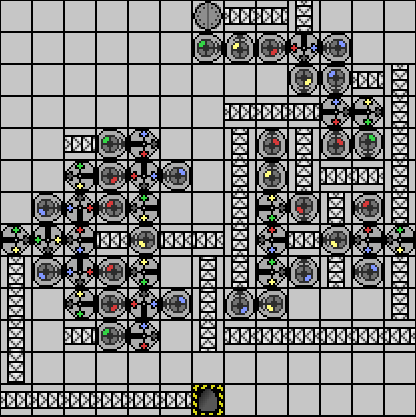
\includegraphics[scale=0.75]{0.png} \par
	\caption{manufactoria游戏界面截图}
\end{figure}
manufactoria游戏为我们提供了一个很好的图形化编程平台的范例。本学期,在学习了《人机交互理论与技术》、《嵌入式系统》等课程后,我们想到了以manufactoria为原型设计一个图形化编程平台的设计方案,将编程语言中的常见语句与模块抽象为图形元件放入网格中,并通过网格中的箭头指示程序执行流程,来构成完整程序。同时,编写的程序可以由用户在图形界面编译成嵌入式开发板支持的代码,并在嵌入式开发板上执行,在显示屏等输出设备上输出结果。\par
我们最初的设计中选用的嵌入式开发板为Arduino Uno,所以本项目命名为\texttt{manuduino}。但设计过程中由于硬件兼容性等问题,我们最终改为以Raspberry Pi 3(树莓派3)作为使用的嵌入式开发板,并以液晶显示器作为输出设备。\par

\section{功能介绍}
\subsection{图形界面(GUI)}
\subsubsection{制造模式(Manu Mode)}
制造模式是本项目的主要模式,其图形界面如下图所示:\par
\begin{figure}[htb]
	\centering 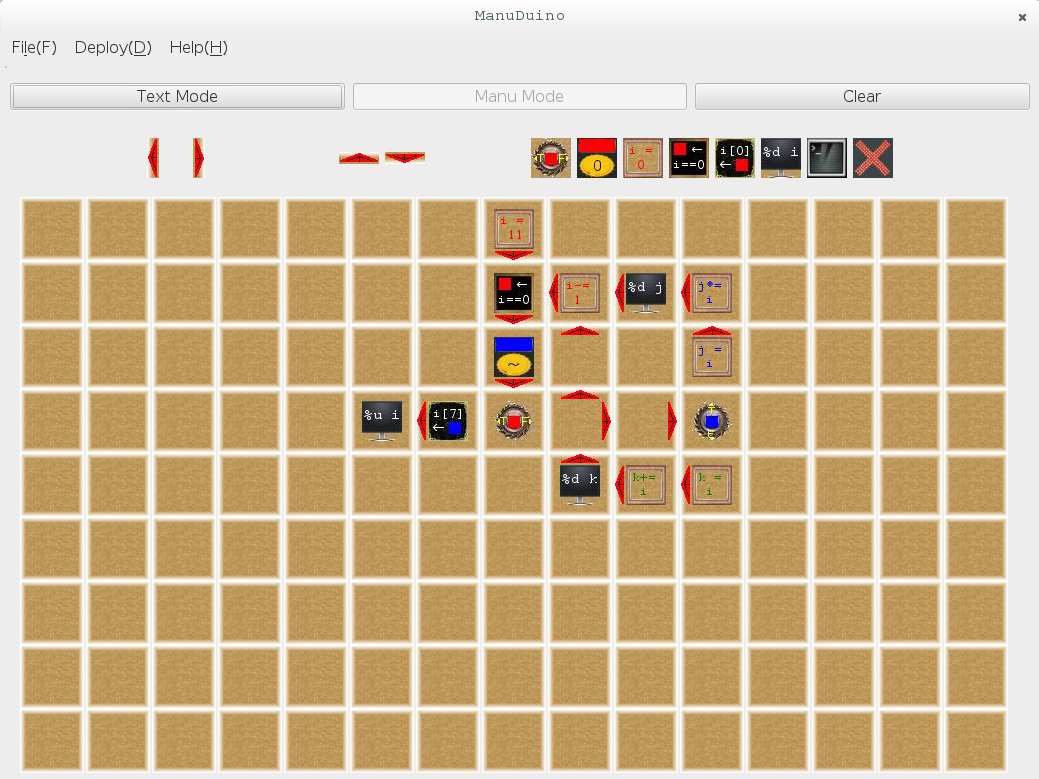
\includegraphics[scale=0.5]{1.png} \par
	\caption{\texttt{manuduino}制造模式图形界面}
\end{figure}
主界面为9行15列的网格,其中每个格子中心处可以放置至多一个中央元件(Central Entity),四周可以放置上/下/左/右四个方向的箭头(Arrow),每个格子中,上下箭头至多一个,左右箭头至多一个。\par
主界面以上为操作菜单栏(Operation Menu),包含上下左右箭头、各种中央元件以及删除操作。用户可以通过\uline{鼠标左键单击}这些元件的图标并用\uline{鼠标拖动}到任意一个格子里来放置这些元件。各个中央元件以及删除操作的说明如下表(对于变量的说明见2.3节):\par \vspace*{1ex}
\begin{tabular}{|c|c|c|c|}
	\hline
	名称 & 图标 & 说明 & 备注 \\
	\hline
	\tabincell{c}{选择器\\(Selector)} & 
\includegraphics[scale=0.5]{Icons/Selector.jpeg} & \tabincell{l}{根据bool变量的值决定走向,为\\True则走T方向,为False则\\走F方向。} & \tabincell{l}{双击菜单栏图标可选择具\\体的bool变量与T、F方向。\\该元件所在格无箭头。}\\
	\hline
	\tabincell{c}{布尔控制器\\(Bool Controller)} & 
\includegraphics[scale=0.5]{Icons/BoolController.jpeg} & \tabincell{l}{给bool变量赋值,可赋为0\\(False)、1(True)或$\sim$(取反)。} & \tabincell{l}{双击菜单栏图标可选择具体\\的bool变量与所赋的值。}\\
	\hline
	\tabincell{c}{整数控制器\\(Int Controller)} & 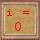
\includegraphics[scale=0.5]{Icons/IntController.jpeg} & \tabincell{l}{给int变量赋值,支持=、\\+=、-=、*=、/=、\%=等\\多种赋值方式,所赋的值可以为\\0$\sim$15的常量或其它int变量。} & \tabincell{l}{双击菜单栏图标可选择具体\\的int变量、赋值方式与\\所赋的值。}\\
	\hline
	\tabincell{c}{比较器\\(Comparator)} & 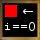
\includegraphics[scale=0.5]{Icons/Comparator.jpeg} & \tabincell{l}{将int变量的值与0比较,并\\将比较结果赋给bool变量,\\比较运算有$=$、$>$、$>=$、\\$<$、$<=$、$!=$等。} & \tabincell{l}{双击菜单栏图标可选择具体\\的int变量、比较方式与\\赋给的bool变量。}\\
	\hline
	\tabincell{c}{置位器\\(Bit Setter)} & 
\includegraphics[scale=0.5]{Icons/BitSetter.jpeg} & \tabincell{l}{将int变量的某一位置为\\某个bool变量的值。} & \tabincell{l}{双击菜单栏图标可选择具体\\的int变量、所置的位与\\bool变量。}\\
	\hline
	\tabincell{c}{输出装置\\(Output)} & 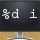
\includegraphics[scale=0.5]{Icons/Output.jpeg} & \tabincell{l}{输出int变量的值,输出格式有\\有符号整型、无符号整型和字符\\型。} & \tabincell{l}{双击菜单栏图标可选择具体\\的int变量与输出格式。}\\
	\hline
	\tabincell{c}{终端\\(Shell)} & 
\includegraphics[scale=0.5]{Icons/Shell.jpeg} & \tabincell{l}{插入自定义代码。\\} & \tabincell{l}{拖动插入终端后,双击可打\\开对话框,输入自定义代码。}\\
	\hline
	\tabincell{c}{删除操作\\(Clear Operation)} & 
\includegraphics[scale=0.5]{Icons/Clear.jpeg} & \tabincell{l}{将其拖动到某个格子内,可删除\\该格所有元件(包括箭头)。} & \\
	\hline
\end{tabular}
\par \vspace*{2ex}
在制造模式中,点击界面上的``Clear"按钮,可清空所有网格。\par

\subsubsection{文字模式(Text Mode)}
本项目除制造模式外,还有一个用于用户测试的文字模式,其界面如下图所示:\par
\begin{figure}[htb]
	\centering 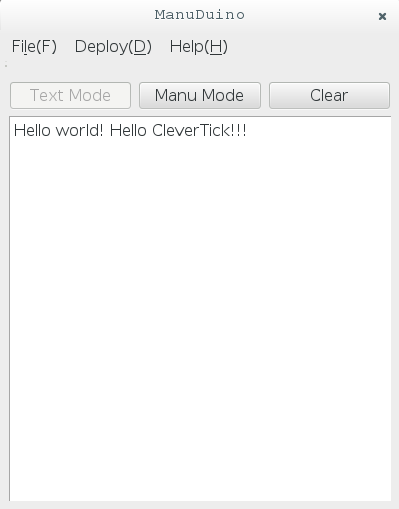
\includegraphics[scale=0.75]{2.png} \par
	\caption{\texttt{manuduino}文字模式界面}
\end{figure}
在文字模式中,用户可直接在文本框内输入文字,执行效果为在显示器上输出文本框内的文字。\par
此模式中点击``Clear"按钮,可清空文本框(不会影响制造模式中的程序)。\par
点击``Manu Mode"与``Text Mode"按钮,可在两种模式间切换。由于文字模式仅用于用户测试,因此本文以下部分,均默认在制造模式下进行。\par

\subsection{程序编译与执行}
在图形界面设计程序之后,需要将程序进行编译,并在嵌入式开发板(Raspberry Pi 3)上执行,在显示屏上输出结果。\par
在Raspberry Pi 3一端上,需要预先安装JRE和processing的ARM版本一边执行,并且需要配置ssh远程登录。在开发端完成图形设计、编译后,之后的部署命令会通过ssh和scp命令自动完成远程的部署和执行。\par

\subsection{运行规则}
\texttt{manuduino}程序中可使用8个bool变量(\uline{用8种不同颜色的色块表示})和3个8位整型(int8)变量(命名为\texttt{i}、\texttt{j}、\texttt{k})。\par
程序运行时,将有一个虚拟的NPC在主界面网格内移动,初始时,其位于第1行第8列(即最上一行中间的格子)上方,初始方向向下(也就是其最先进入的格子为第1行第8列)。所有变量初始值均为False(bool变量)/0(int变量)。\par
程序运行过程中,该虚拟NPC每到达一个格子,就会根据该格的中央元件指示,执行相应操作(如某一格中央元件为写有\texttt{i=11}的整数控制器,则NPC到达该格后,会执行将变量\texttt{i}的值赋为11的操作),若该格没有任何中央元件,则什么也不做。之后,NPC会根据该格含有的箭头方向,决定其下一步的走向(对于中央元件是选择器的格子,则根据选择器的结果决定下一步走向):
\begin{itemize}
    \item 若该格含有两个箭头(上下箭头、左右箭头各一个),则当NPC上一步走进该格时的方向为上/下方向,则下一步走上/下箭头指示的方向;当NPC上一步走进该格时的方向为左/右方向,则下一步走左/右箭头指示的方向;
    \item 若该格只有一个箭头,则不论NPC上一步走进该格时是什么方向,下一步均走这个箭头指示的方向;
    \item 若该格没有箭头(中央元件是选择器的格子除外),或者NPC走出了网格区,则程序立即终止(除此以外,没有其它办法能让程序终止)。
\end{itemize}

\section{设计详情}
\subsection{模块划分}
本项目主要在Qt 4开发环境下编写,以Raspberry Pi 3作为嵌入式开发板(用于执行程序)。整个项目划分为以下模块:
\begin{itemize}
	\item 元件(Entity类):定义图形界面中用到的各种图形元件,其派生类有Arrow(定义箭头)、EmptyEntity(定义空元件)、OperationEntity(定义菜单栏操作元件)等;
	\item 中央元件对话框(*Dialog类):定义各种中央元件双击后弹出的对话框内容;
	\item 主界面网格(BoardGrid类):定义主界面的网格,每个格子由3行3列的9个元件(Entity)构成,其中左上、右上、左下、右下元件均固定为空,上中、左中、右中、下中元件留给箭头使用(无箭头时为空),最中间的为中央元件。网格类提供用户操作的主要接口(放置元件、删除等),也为编译器调取主界面局面信息提供接口。
	\item 图形界面主窗口(MainWindow类):定义图形界面的主窗口布局,以及读取用户鼠标操作事件(单击、双击、释放、拖动等)并处理;
	\item 编译器(Compiler类):定义了编译制造模式和文字模式到Java代码的算法。细节见后文描述。
	\item 远程部署(RemoteManager类):自动通过SSH,向连接无线网络的树莓派远程进行部署和执行。
	\item 服务器配置(ServerConfigurationDialog类):用于通过图形界面调整配置远程服务器的相关参数。
\end{itemize}

\subsection{一些设计细节和技巧}
\subsubsection{鼠标拖动效果的设计}
为了增强交互效果,本项目实现了一个重要的功能——将元件用鼠标左键拖动到网格内。\par
Qt中鼠标拖动的事件处理集成在鼠标移动(\texttt{mouseMoveEvent()})中,这样就无法判断鼠标指针移动操作是否在点击操作元件之后发生。为了解决这个问题,我们利用Qt的“信号——槽”机制,设计了“激活”机制——在OperationEntity类中进行鼠标按下事件(\texttt{mousePressEvent()})处理,当用户按下了操作菜单栏上的某个元件图标时,就发射“该元件被激活”的信号,主窗口类MainWindow的一个槽接收该信号,判定这个元件被激活。此后在鼠标移动时,鼠标指针(用QCursor控制)会被置为目前被激活的元件(如果有的话),以实现“拖动”效果。\par
\subsubsection{鼠标释放事件处理机制}
在主界面中,当用户拖着某个元件至某处释放鼠标左键时,需要判断该释放处是否为某个网格内部,若是则在该网格中加入元件,若否则什么也不做。因此,在处理鼠标释放事件时,我们需要读取该释放事件发生的全局坐标(即鼠标指针当前在主窗口中的位置),并调用网格(BoardGrid)类的\texttt{mapToGlobal()}接口,获取每个网格的坐标范围,以确定释放处是否位于及位于哪个网格当中。\par
\subsubsection{编译、执行的实现细节}
编译过程是这样进行的。首先,“终端”模块允许用户插入任意processing(Java)代码,但是全局变量的定义显然必须脱离控制流,因此,定义扩展关键字“__global;”,以此行开头的终端代码会被调整到整个processing
程序的变量定义段。接下来程序生成其运行时代码。利用processing的变量定义个setup函数,整个网格中所有的箭头信息都被转化为一个Java数组存储。而程序的真正执行是通过在processing的draw函数中以状态机
模式来运行。每一次经过自动循环的draw函数,都会执行为坐标匹配的manuduino模块编译出的代码。除此之外,编译器还创建了一段运行时环境代码,用于根据之间存储的网格信息和选择器信息决定网格位置的移动,
以及在执行到没有箭头的位置之后自动停机。 \par
编译完成之后,程序通过ssh和scp命令,配合一个图形化的SSH AskPass程序,像远程服务器传输创建目录和复制文件的命令。最后,当用户要求执行代码时,则通过ssh命令配置X服务器连接信息并执行
编译好的processing程序。

\section{项目测试及其结果}
参见本报告所在目录中的视频附件。

\section{代码仓库}
在开发本项目的过程中,我们使用Git进行版本控制与代码的维护工作。代码仓库位于Github上,地址为:\par
\texttt{https://github.com/MatoNo1/manuduino.git}

\end{document}
